% Provenance (never printed): old terminale S material on past climates (ice cores,
% pollen, ocean sediments and oxygen isotopes, glacial-interglacial cycles, the
% astronomical rhythm told, climates of deep time), read from data. Owner (Sync 0/1):
% climate archive and proxy, ice core, glacial period, interglacial and glacial cycle,
% pollen analysis, Last Glacial Maximum. Recalled: glacier, ice sheet, ice age (Book 1,
% grade 8); the first look at the ice-core records (Book 1, grade 9); isotopes
% (physics); greenhouse gases (chemistry); the time scale (Book 1, grade 7). The
% delta notation of isotopes is Book 3's: isotope curves are read here as told,
% without a definition. The orbital theory of climate belongs to a university book:
% told here only. Physical science only, in the IPCC's calibrated words.
% Figures: figdata/grade-12/ice_age_records.py (tests/grade-12/test_ice_age_records.py).
\chapter{读取过去的气候}\label{ch:g12:past-climates}

在 Dome~C 站，位于东南极冰盖上、海拔 \qty{3233}{m} 处，空气
年平均温度约为 \qty{-55}{\degreeCelsius}。一台钻机在那里
钻至 \qty{3260}{m} 深处停止，此处距冰下基岩约 \qty{15}{m}。
所取出的最深冰层中含有微小的气泡，
年龄约为 \num{800000} 年，是远在最早的农夫出现之前的大气样本。
本章
从冰层、湖泊与海底的淤泥以及岩石中读取过去的气候，
并探讨这些信息对今天有何启示。
% ledger: ipev:concordia, edc3:drilling, jouzel07:edc

\begin{omfigure}
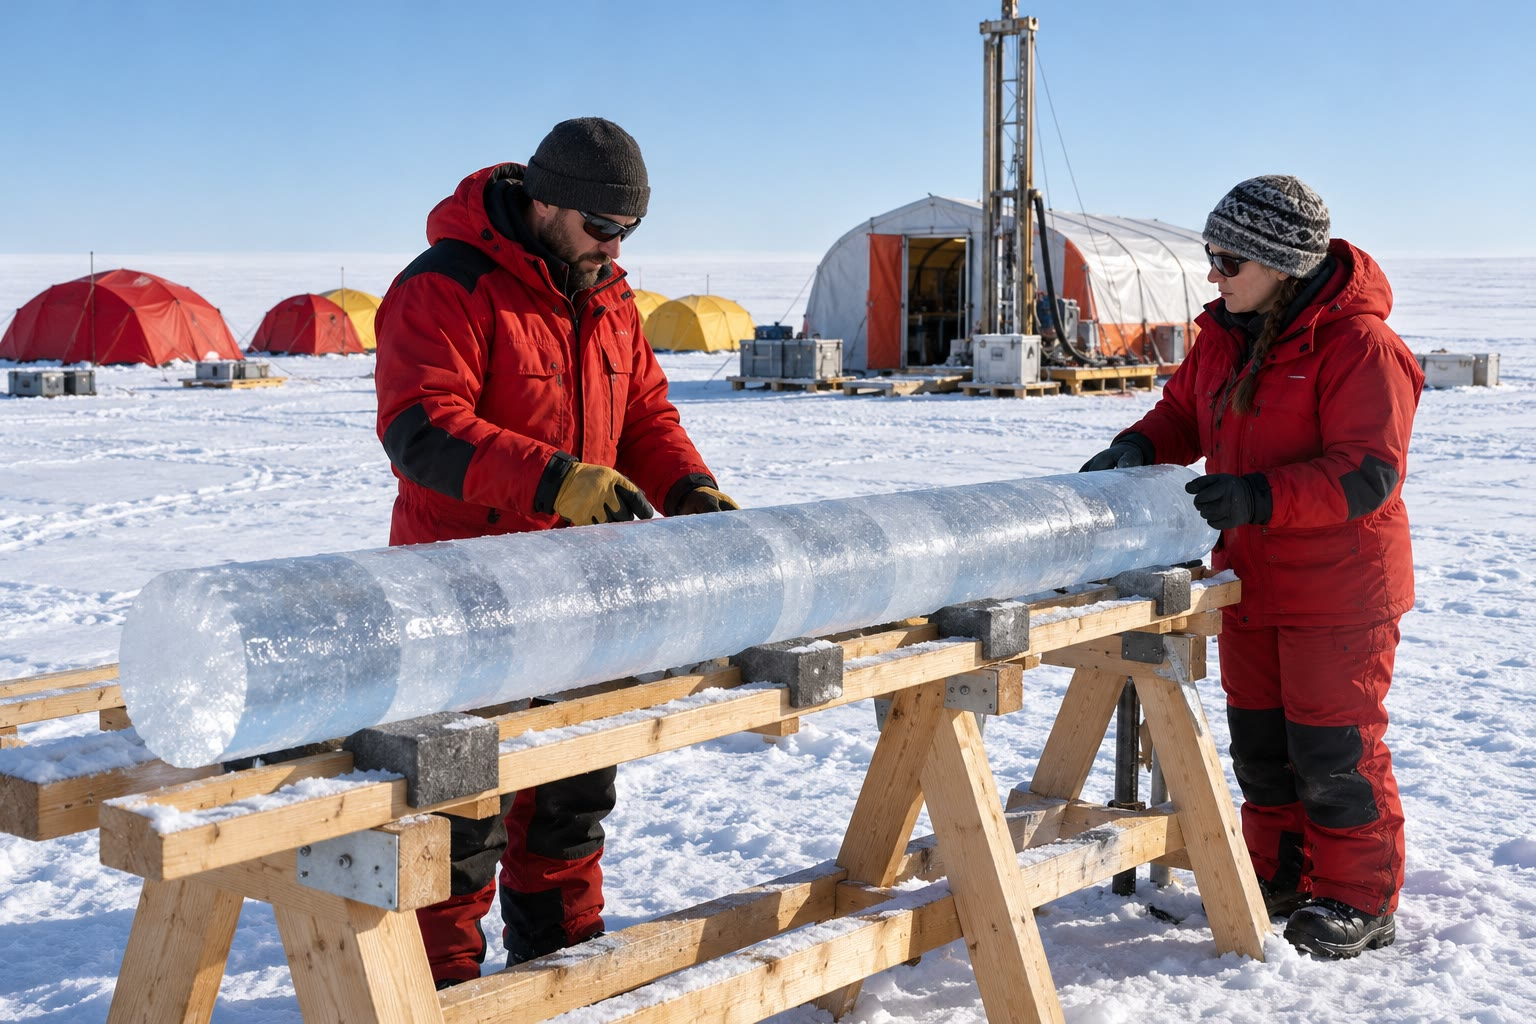
\includegraphics[width=0.56\linewidth]{images/book2/ai/g12-ice-coring-camp.jpg}

{\small 极地冰盖上的\omterm{def:g12:past-climates:ice-core}{冰芯}钻探营地：钻机在塔架与
棚屋下工作，每段岩芯取出后都被摆放、记录并
装箱，然后运往实验室。AI 生成插图。}
\end{omfigure}

\begin{recall}
冰川是一种年复一年存在、在自身重力下流动的冰体；
冰盖覆盖大陆的大部分区域；\omterm{def:g12:past-climates:glacial-cycle}{冰期}是漫长的寒冷时期，
此时冰盖远远扩展到两极之外（见第 1 册，八年级）。
在南极\omterm{def:g12:past-climates:ice-core}{冰芯}中，雪记录了空气温度，气泡保存了空气本身，
两种记录的升降趋势一致（见第 1 册，九年级）。
同一元素的原子可能因中子数不同而有所差异：
这些同位素化学性质相近，但质量不同（参见
物理各册）。二氧化碳是一种温室气体（参见化学各册）。
第四纪开始于 258 万年前
（见第 1 册，七年级）。
\end{recall}
% ledger: ics:base.Quaternary (shared), nasaeo:o18 (snow poor in heavy isotopes)

\section{档案与代用指标}

没有人测量过 \num{20000} 年前的空气温度。但地球
在无意之中保存了记录：冰层与淤泥、贝壳与树干，
它们各自都随形成时的气候而变化。

\begin{definition}[气候档案；代用指标]\label{def:g12:past-climates:proxy}
称\emph{气候档案}\index{气候档案}为一种天然材料，它按层逐一沉积，
保存着形成时气候的痕迹：极地冰层、湖泊与海底的沉积物、
树木年轮、珊瑚、洞穴沉积物等。
称\emph{代用指标}\index{代用指标}为档案中测得的一个量，
用以代替某个未曾测量的气候变量：老雪中重同位素的比例
代表空气温度，
湖泊淤泥中各类花粉的比例代表植被，
进而代表气候。
\end{definition}
% ledger: ncei:proxy, ncei:pollen, nasaeo:o18

\begin{center}
\small
\begin{tabular}{|l|l|l|}
\hline
\textbf{档案} & \textbf{\omterm{def:g12:past-climates:proxy}{代用指标}} & \textbf{反映的内容} \\
\hline
极地冰 & 冰中的重同位素 & 冰面上方的空气温度 \\
 & 气泡中的空气 & 二氧化碳、甲烷 \\
湖泊沉积物、泥炭 & 花粉 & 植被，进而是气候 \\
海洋沉积物 & 贝壳中的氧同位素 & 冰量、深层海水温度 \\
树木年轮 & 年轮宽度 & 逐年的生长条件 \\
珊瑚、洞穴沉积物 & 同位素、生长带 & 海水或空气温度、降雨 \\
\hline
\end{tabular}

\medskip
{\small 主要\omterm{def:g12:past-climates:proxy}{气候档案}及其部分\omterm{def:g12:past-climates:proxy}{代用指标}。}
\end{center}
% ledger: ncei:proxy, nasaeo:o18

\omterm{def:g12:past-climates:proxy}{代用指标}在被读取前需要两个条件。其一是\emph{时钟}：
即各层的年龄，可由可见处的逐年层位计数得出，
或由放射性测年（见\cref{ch:g12:age-of-the-earth}），或由将记录与
另一已测定年代的记录相对照得出。还需要\emph{校准}：
测得量与气候变量之间的联系，
由今天两者可以同时测量之处求得。

\begin{method}[读取代用指标记录]
\begin{enumerate}
  \item 找出档案与\omterm{def:g12:past-climates:proxy}{代用指标}：测量的是什么，以及在何种材料中测量？
  \item 找出坐标轴上时间的方向及单位；检查
        \omterm{def:g12:past-climates:proxy}{代用指标}的坐标轴是否反向。
  \item 解读\omterm{def:g12:past-climates:proxy}{代用指标}：数值越大表示更暖还是更冷，
        冰量更多还是更少？
  \item 注意样品的间隔：数据点之间
        相隔 \num{2000} 年的记录，无法显示持续一个世纪的变化。
  \item 读取指定时刻的数值，或某一时段的平均值，
        并计算变化量与变化速率。
  \item 先说明记录在其所在地点反映了什么，然后再判断
        它能否代表整个地球。
\end{enumerate}
\end{method}

\section{冰芯}

\begin{definition}[冰芯]\label{def:g12:past-climates:ice-core}
称\emph{冰芯}\index{冰芯}为从冰盖或冰川中钻取的圆柱状冰体。
其深度给出冰的年龄，越深则越古老；
冰记录了降雪时空气的温度，
其中的气泡保存了当时空气的样本。
\end{definition}
% ledger: ncei:proxy, jouzel07:edc

新降的雪大部分是空气。埋在随后数年的积雪之下，它
压实为\emph{粒雪}，即孔隙仍能透气的压实雪。
密度约为 820 至 \qty{830}{kg/m^3}，埋深 50 至 \qty{120}{m}
时，孔隙闭合，空气被封存于气泡中。因此冰保存了两种不同的
记录。气泡中的空气是大气的样本，其二氧化碳
与甲烷可在实验室中测定。冰本身则保存了
温度信息：含有重同位素（氘或
氧-18）的水分子比轻的更易凝结，因此
在通往极地的途中空气越冷，降雪中的重同位素就越少。
% ledger: firn:close-off, nasaeo:o18

\begin{omfigure}
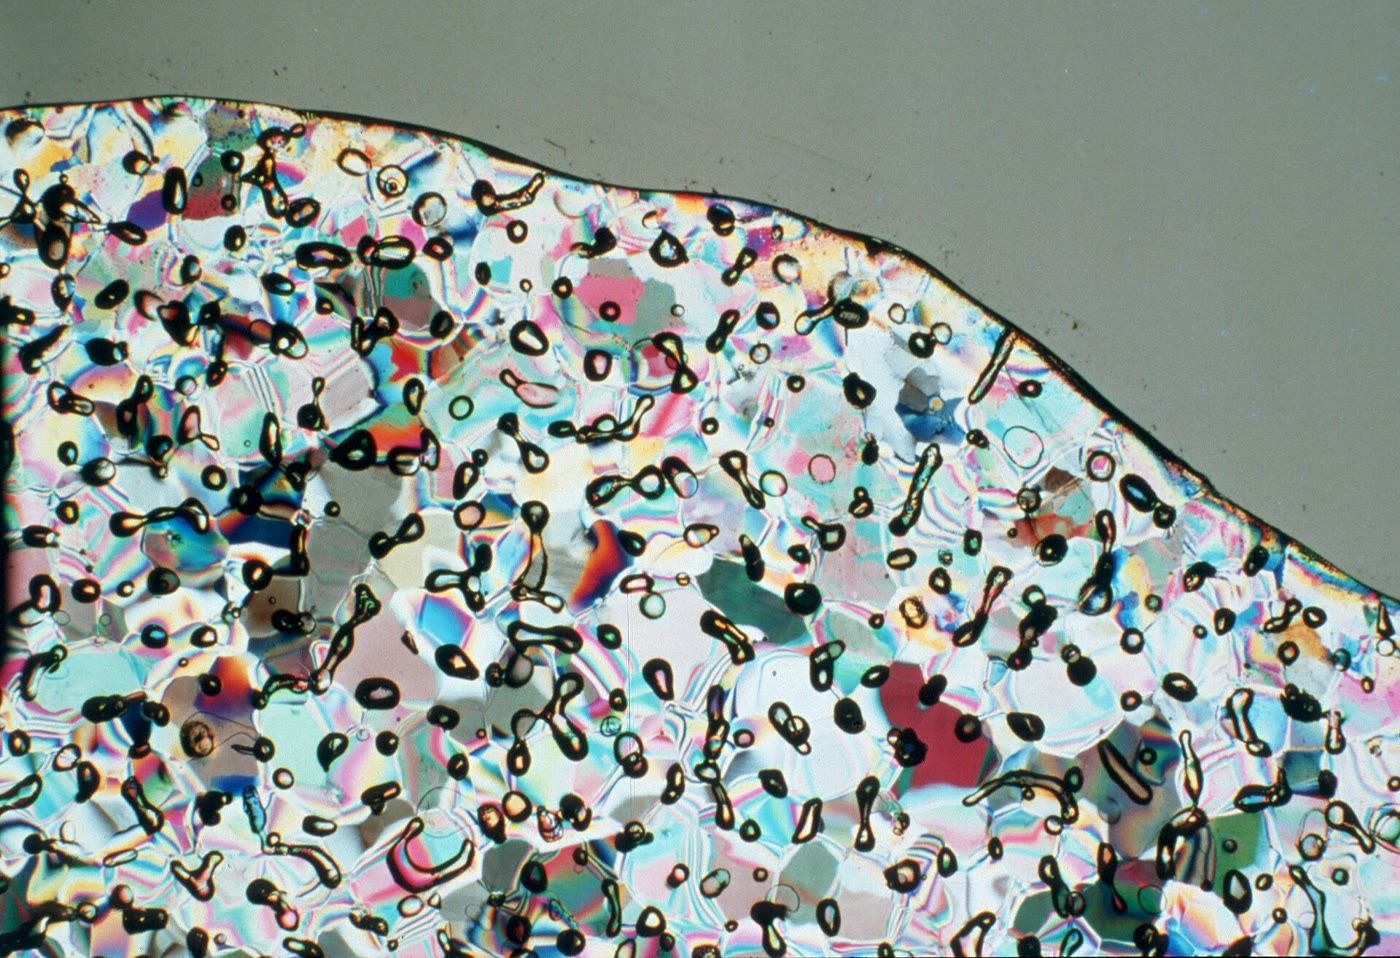
\includegraphics[width=0.50\linewidth]{images/book2/g12-ice-bubbles.jpg}

{\small 偏振光下所见的南极冰片，偏振光使冰晶呈色；
暗色斑点为被封存的空气气泡。照片：CSIRO
Atmospheric Research, CC~BY~3.0（维基共享资源）。}
\end{omfigure}
% ledger: photo:g12-ice-bubbles

Dome~C \omterm{def:g12:past-climates:ice-core}{冰芯}中的氘已换算为
冰面上方的温度，以其相对最近一千年平均值的变化量表示。
二氧化碳取自若干南极\omterm{def:g12:past-climates:ice-core}{冰芯}的气泡，
合并为一条记录。两者均绘于下图同一时间轴上。

\begin{omfigure}
\begin{tikzpicture}
\begin{axis}[omrecord, scale only axis, width=0.74\linewidth, height=4.8cm,
  xmin=0, xmax=800, x dir=reverse, ymin=-12, ymax=8, axis y line*=left,
  xtick={0,100,...,800}, ytick={-10,-5,0,5},
  xlabel={1950 年以前的千年数},
  ylabel={温度变化（\unit{\degreeCelsius}）}]
% data:edc-jouzel, 2-kyr means (figdata/grade-12/ice_age_records.py)
\addplot[omWarm, line width=0.7pt] table[x=age_kyr, y=temp_C] {figdata/out/grade-12-ice_age_records-edc.dat};
\end{axis}
\begin{axis}[scale only axis, width=0.74\linewidth, height=4.8cm,
  xmin=0, xmax=800, x dir=reverse, ymin=60, ymax=320, axis y line*=right,
  axis x line=none, ytick={180,220,260,300}, ylabel={二氧化碳（ppm）},
  every axis label/.append style={font=\small}, tick label style={font=\small}]
% data:co2-bereiter, 2-kyr means
\addplot[black, line width=0.7pt] table[x=age_kyr, y=co2_ppm] {figdata/out/grade-12-ice_age_records-co2.dat};
\coordinate (lt) at (axis cs:560,70);
\coordinate (lc) at (axis cs:560,312);
\end{axis}
\node[font=\scriptsize, text=omWarm, anchor=south] at (lt) {Dome~C 处温度（左侧刻度）};
\node[font=\scriptsize, anchor=north] at (lc) {二氧化碳（右侧刻度）};
\end{tikzpicture}

{\small 八十万年的南极\omterm{def:g12:past-climates:ice-core}{冰芯}记录，按
\num{2000}~年为步长取平均。红色：Dome~C 处温度，相对最近一千年
的变化（Jouzel 等，2007）；黑色：气泡中的二氧化碳
（Bereiter 等，2015）。今日位于右侧。}
\end{omfigure}
% ledger: data:edc-jouzel, data:co2-bereiter

两条曲线呈现同一规律：缓慢起伏地滑向寒冷，
历经数万年，随后快速回升至温暖，
再次滑向寒冷。

\begin{definition}[冰期；间冰期；冰期旋回]\label{def:g12:past-climates:glacial-cycle}
\emph{冰期}\index{冰期}是冰期之内的一段寒冷时段，
此时冰盖远大于今日的规模。\emph{间冰期}\index{间冰期}是
两次冰期之间的一段温暖时段，
冰盖接近今日规模或更小；今日正处于其中，
它始于约 \num{11000}~年前。一个\emph{冰期
旋回}\index{冰期旋回}是一个冰期，
连同终结该冰期的间冰期。
\end{definition}
% ledger: ipcc:ref-periods (LDT ends 11 ka); the count of cycles is read from the figure (data:edc-jouzel)

全部记录中，Dome~C 处温度的变化范围从
\qty{-10.6}{\degreeCelsius}（约 \num{24000}~年前）至
\qty{+5.5}{\degreeCelsius}（约 \num{129000}~年前）；二氧化碳浓度则
从 \qty{174}{ppm} 变化至 \qty{299}{ppm}。图中数据经 \num{2000}~
年平均，略微平滑了这些极值。统计温暖峰值，得到八个或九个
\omterm{def:g12:past-climates:glacial-cycle}{冰期旋回}；温度记录中最强的节律，
由其数据计算得出，周期约为 \num{98000}~年。
% ledger: data:edc-jouzel, data:co2-bereiter (ice_age_records.py: edc_min_C -10.58 at 24.0 kyr, edc_max_C 5.46 at 128.7 kyr, co2 173.71 and 298.6, edc_period_kyr 97.5)

\begin{proposition}[温度与二氧化碳同步变化]\label{prop:g12:past-climates:correlation}
% ledger: data:edc-jouzel, data:co2-bereiter (ice_age_records.py: r_temp_co2 0.9165, fit 266.57 + 7.827 T, 1639 pairs)
过去 \num{800000}~年间，南极温度与大气中的二氧化碳
同步变化。将 1639 个距今超过 \num{2000}~年的二氧化碳测量值，
各与同龄的 Dome~C 温度配对，
得相关系数 $r = 0.92$，并给出
最小二乘直线
\[
  \mathrm{CO_2} \approx \qty{267}{ppm} + \qty{7.8}{ppm/\degreeCelsius} \times \Delta T ,
\]
其中 $\Delta T$ 为 Dome~C 处的温度变化。
\end{proposition}

\begin{proof}[计算方法]
对每个二氧化碳样本，其所对应年龄的温度，在
Dome~C 记录中由最近的两个温度数据点插值得到。
1639 组数据的相关系数是介于 $-1$ 与 $1$ 之间的数，
它刻画数据点与直线的接近程度（参见数学教材），
由最小二乘直线算得；两者均在绘图脚本中计算，
并经其测试程序校验。
\end{proof}

\begin{omfigure}
\begin{tikzpicture}
\begin{axis}[omrecord, width=0.70\linewidth, height=5.2cm, xmin=-12, xmax=6,
  ymin=160, ymax=310, xlabel={Dome~C 处温度变化（\unit{\degreeCelsius}）},
  ylabel={二氧化碳（ppm）}]
% data:edc-jouzel, data:co2-bereiter (pairs and fit in ice_age_records.py)
\addplot[only marks, mark=*, mark size=0.6pt, omDef, opacity=0.45] table[x=temp_C, y=co2_ppm] {figdata/out/grade-12-ice_age_records-pairs.dat};
\addplot[omThm, line width=1pt] table[x=temp_C, y=co2_ppm] {figdata/out/grade-12-ice_age_records-fit.dat};
\node[font=\scriptsize, text=omThm, anchor=south east, fill=white, inner sep=1pt] at (axis cs:-1.5,295) {最小二乘直线，$r = 0.92$};
\end{axis}
\end{tikzpicture}

{\small 每个点是南极\omterm{def:g12:past-climates:ice-core}{冰芯}中的一次二氧化碳测量，
按同一时代的 Dome~C 温度标在图上：冷期的二氧化碳很少，
暖期则多得多。由 Jouzel 等人（2007）和
Bereiter 等人（2015）的数据计算得出。}
\end{omfigure}

相关性并不能说明哪一个先变化，也不能说明是否有第三个因素
同时推动了两者：若温度驱动二氧化碳，若二氧化碳驱动温度，
或二者相互推动，相关系数都相同。
约 \num{100000} 年的节律由何种因素决定，将在下文关于海洋的一节中说明，
二氧化碳如何影响温度，
则在\cref{ch:g12:climate-change}中讨论。

\subsection{末次盛冰期}

\begin{definition}[末次盛冰期]\label{def:g12:past-climates:lgm}
称\emph{末次盛冰期}\index{末次盛冰期}为距今约
\num{23000} 至 \num{19000} 年前，末次\omterm{def:g12:past-climates:glacial-cycle}{冰期}的冰盖
范围最大的时期。
\end{definition}
% ledger: ipcc:ref-periods

\omterm{def:g12:past-climates:lgm}{末次盛冰期}时，冰盖覆盖了北美洲大部分和欧亚大陆西北部，
当时的气候比今天更干燥、多尘。
评估认为，\omterm{def:g12:past-climates:lgm}{末次盛冰期}的全球表面温度比 1850--1900 年低 \qty{5}{\degreeCelsius}
至 \qty{7}{\degreeCelsius}（\emph{中等可信度}），
二氧化碳浓度为 188 至 \qty{194}{ppm}。冰盖中锁存的水
来自海洋：全球平均海平面
比今天低 125 至 \qty{134}{m}。
% ledger: ipcc:ref-periods, ipcc:lgm-cooling, ipcc:fig2-34, ipcc:lgm-sea, lambeck14:lgm

海平面降低会使大陆周围的浅海底裸露。下图将海平面降低
\qty{130}{m}（即上述范围的中值），
底图为今日东南亚的地形。

\begin{omfigure}
\begin{tikzpicture}
\begin{axis}[omrecord, axis equal image, width=0.62\linewidth, xmin=92, xmax=122,
  ymin=-11, ymax=24, grid=none, axis x line=box, axis y line=box,
  xtick={95,105,115}, ytick={-10,-5,...,20},
  xticklabel={\pgfmathprintnumber{\tick}\textdegree E},
  yticklabels={10\textdegree S, 5\textdegree S, 0\textdegree, 5\textdegree N, 10\textdegree N, 15\textdegree N, 20\textdegree N}]
% data:b2-etopo-sunda (raster computed in ice_age_records.py; sea level lowered by 130 m)
\addplot graphics[xmin=91.95, xmax=122.05, ymin=-11.05, ymax=24.05] {figdata/out/grade-12-ice_age_records-sunda.png};
\node[font=\scriptsize] at (axis cs:114.5,0.5) {婆罗洲};
\node[font=\scriptsize, rotate=-45] at (axis cs:101.9,-1.3) {苏门答腊};
\node[font=\scriptsize] at (axis cs:110.5,-8.6) {爪哇};
\node[font=\scriptsize, rotate=-60] at (axis cs:102.2,4.0) {马来半岛};
\node[font=\scriptsize] at (axis cs:103,16.5) {中南半岛};
\node[font=\scriptsize, align=center] at (axis cs:106.5,3.5) {巽他 \\陆架};
\node[font=\scriptsize, align=center] at (axis cs:114.5,13) {南海};
\node[font=\scriptsize, align=center] at (axis cs:96,-6) {印度 \\洋};
\end{axis}
\end{tikzpicture}

{\small 海平面比今天低 \qty{130}{m} 时的东南亚。绿色：
今日陆地；棕褐色：海平面降低 \qty{130}{m} 后裸露的海底；蓝色：
海。底图采用现今地形，因此海岸线仅为近似。
由 ETOPO1 地形数据（NOAA）计算得出，每 0.1 度取一点。}
\end{omfigure}
% ledger: data:b2-etopo-sunda, ipcc:lgm-sea

婆罗洲、苏门答腊和爪哇与马来半岛、
中南半岛连成一片：巽他陆架今天位于浅海之下，当时是陆地。图上可见，
海平面仅降约 \qty{36}{m}，婆罗洲即与亚洲相连，苏门答腊与
爪哇相连更早。图上可见，
海面以上陆地面积由 4.11 增至 7.16 百万平方千米，
为原来的 1.74 倍。全球范围内，同样下降 \qty{130}{m} 的海平面，使
海面以上地表所占比例由 \qty{29.0}{\percent} 升至
\qty{33.5}{\percent}，新增陆地约 2300 万平方千米。
% ledger: data:b2-etopo-sunda, data:etopo1 (ice_age_records.py: borneo_link_m -36; sunda_land_now_km2 4.105e6, lgm 7.161e6, ratio 1.744; world_land_now_frac 0.2904, lgm 0.3352, world_gain_km2 2.285e7)

\begin{example}[末次冰消期]
\omterm{def:g12:past-climates:lgm}{末次盛冰期}之后的变暖称为末次
冰消过渡期；评估认为其大致位于 \num{18000} 至
\num{11000} 年前之间。在 Dome~C 记录中，\omterm{def:g12:past-climates:lgm}{末次盛冰期}的平均温度
（\num{23000} 至 \num{19000} 年前）为
\qty{-9.4}{\degreeCelsius}；随后 \num{11000} 至
\num{9000} 年前区间的平均值为 \qty{-0.4}{\degreeCelsius}。南极上空的气温
升高了 \qty{9.0}{\degreeCelsius}，二氧化碳浓度由
\qty{190}{ppm} 升至 \qty{264}{ppm}，增加 \qty{74}{ppm}。全球范围内，
变暖幅度与评估所得的 5 至 \qty{7}{\degreeCelsius} 降温相当，约
\qty{6}{\degreeCelsius}，分布于该过渡期的 \num{7000} 年间：
\[
  \frac{\qty{6}{\degreeCelsius}}{\num{7000}\ \text{年}} \approx
  \qty{0.86}{\degreeCelsius} \text{ 每千年.}
\]
同期海平面由约 \qty{-120}{m} 升至 \qty{-50}{m}，
平均每年上升约 \qty{10}{mm}。
\end{example}
% ledger: ipcc:ref-periods, ipcc:lgm-cooling, ipcc:lgm-sea, data:edc-jouzel, data:co2-bereiter (ice_age_records.py: edc_lgm_C -9.389, edc_holo_C -0.360, rise 9.029; co2 189.67, 264.10, rise 74.43; ldt_mean_rate 0.857)

\begin{omfigure}
\begin{tikzpicture}
\begin{axis}[omrecord, scale only axis, width=0.74\linewidth, height=4.6cm,
  xmin=0, xmax=30, x dir=reverse, ymin=-11, ymax=12, axis y line*=left,
  xtick={0,5,...,30}, ytick={-10,-5,0},
  xlabel={1950 年以前的千年数},
  ylabel={温度变化（\unit{\degreeCelsius}）}]
\fill[omDef!10] (axis cs:23,-11) rectangle (axis cs:19,12);
\fill[omProp!12] (axis cs:18,-11) rectangle (axis cs:11,12);
% data:edc-jouzel, every sample
\addplot[omWarm, line width=0.6pt] table[x=age_kyr, y=temp_C] {figdata/out/grade-12-ice_age_records-edc30.dat};
\coordinate (lgm) at (axis cs:21,11.6);
\coordinate (ldt) at (axis cs:14.5,11.6);
\coordinate (lt) at (axis cs:5.5,-3.6);
\end{axis}
\begin{axis}[scale only axis, width=0.74\linewidth, height=4.6cm,
  xmin=0, xmax=30, x dir=reverse, ymin=60, ymax=290, axis y line*=right,
  axis x line=none, ytick={200,240,280}, ylabel={二氧化碳（ppm）},
  every axis label/.append style={font=\small}, tick label style={font=\small}]
% data:co2-bereiter, every sample
\addplot[black, line width=0.6pt, mark=*, mark size=0.5pt] table[x=age_kyr, y=co2_ppm] {figdata/out/grade-12-ice_age_records-co230.dat};
\coordinate (lc) at (axis cs:26.5,196);
\end{axis}
\node[font=\scriptsize, anchor=north, align=center] at (lgm) {末次盛 \\冰期};
\node[font=\scriptsize, anchor=north, align=center] at (ldt) {末次冰消 \\过渡期};
\node[font=\scriptsize, text=omWarm, anchor=north] at (lt) {温度（左）};
\node[font=\scriptsize, anchor=south] at (lc) {二氧化碳（右）};
\end{tikzpicture}

{\small Dome~C 过去 \num{30000} 年的全部测量：
温度（红色）与二氧化碳（黑色）一同自\omterm{def:g12:past-climates:lgm}{末次盛冰期}起上升。
\omterm{def:g12:past-climates:lgm}{末次盛冰期}。阴影部分为\omterm{def:g12:past-climates:lgm}{末次盛冰期}与末次冰消
过渡期，依 IPCC 定年。数据来源：Jouzel 等（2007）、Bereiter
等（2015）。}
\end{omfigure}
% ledger: data:edc-jouzel, data:co2-bereiter, ipcc:ref-periods

\section{花粉}

每年春季，植物都会释放大量花粉。其中大部分散失了，但有一些
落到湖泊和沼泽中，沉入水底，被埋在泥中，保存着
周围植被的记录。每一类
植物的花粉粒都有各自的形状与大小。
% ledger: ncei:pollen

\begin{omfigure}
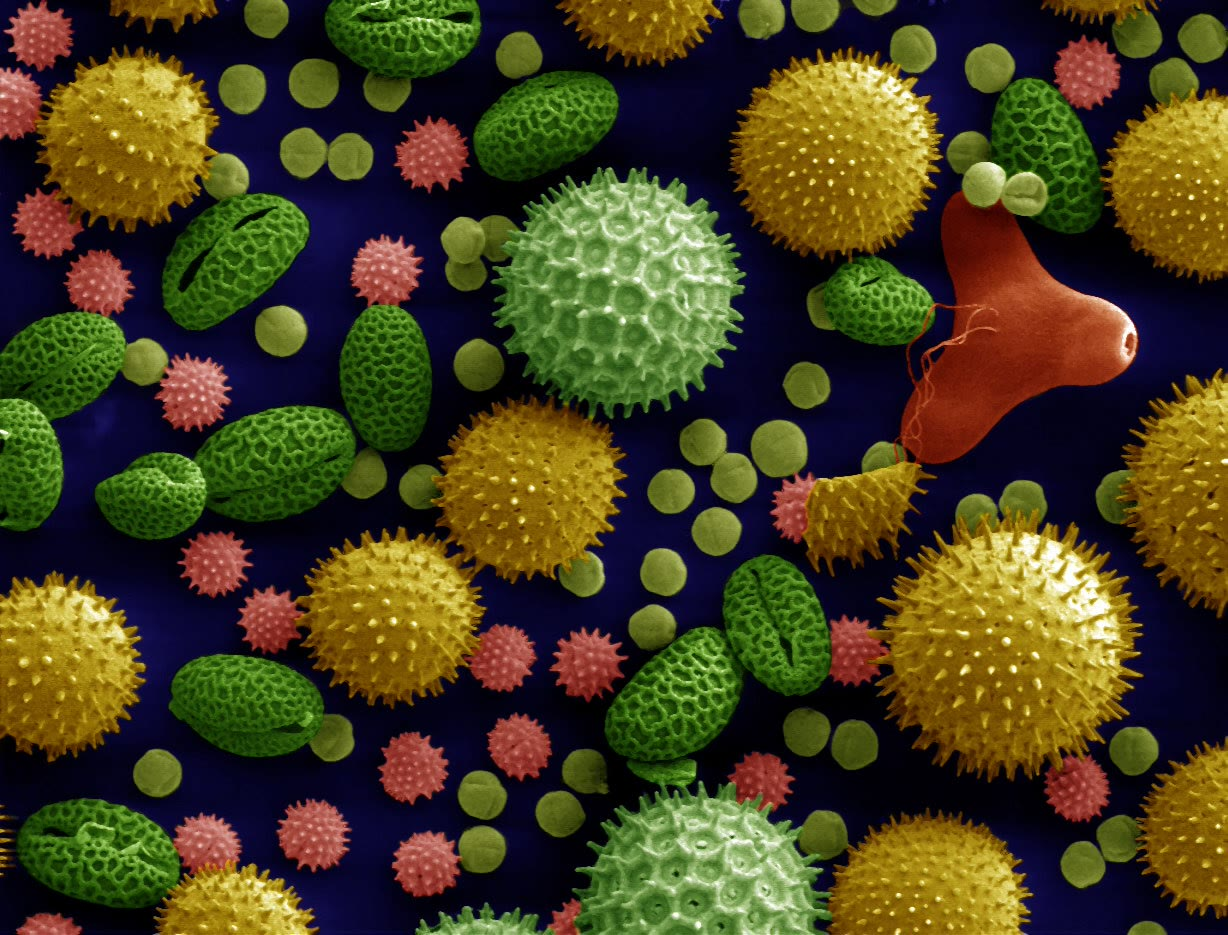
\includegraphics[width=0.46\linewidth]{images/book2/g12-pollen-sem.jpg}

{\small 五种常见植物的花粉粒（向日葵、牵牛花、
蜀葵、百合和报春花）经扫描电子显微镜观察，并着以
假色。每种植物的花粉粒形状各异。Dartmouth
Electron Microscope Facility（公有领域，经由维基共享资源）。}
\end{omfigure}
% ledger: photo:g12-pollen

\begin{definition}[孢粉分析]\label{def:g12:past-climates:pollen}
\emph{孢粉分析}\index{孢粉分析}是解读过去
植被的方法：依据沉积物中保存的花粉，在岩芯的每一层中，
花粉粒被鉴定并计数，各类植物所占的份额，
以所计花粉粒的百分比表示，随深度绘制在
\emph{孢粉图谱}\index{孢粉图谱}中。
\end{definition}
% ledger: ncei:pollen

这种花粉计数方法始于瑞典地质学家伦纳特·冯·
波斯特，他于 1916 年给出了第一幅带数值的现代\omterm{def:g12:past-climates:pollen}{孢粉图谱}；
这种图谱沿页面向下表示深度，每一种植物对应一条曲线。
植被又能说明气候：禾草及其他草本植物
几乎不见树木，意味着开阔、寒冷的景观；而栎树和
榛树则需要温暖的夏季。
% ledger: rull18:von-post; the Varden diagram is invented (ice_age_records.py POLLEN)

\begin{omfigure}
\begin{tikzpicture}
\pgfplotsset{pollen/.style={scale only axis, height=6cm, ymin=300, ymax=600,
  y dir=reverse, xmin=0, axis x line*=bottom, axis y line*=left, axis line style={-},
  tick label style={font=\scriptsize}, title style={font=\small, yshift=-4pt, text depth=0.25ex, text height=1.6ex},
  ytick={300,350,...,600}, xmajorgrids, ymajorgrids,
  grid style={gray!22, line width=0.3pt}}}
\begin{axis}[pollen, name=p1, width=3.0cm, xmax=100, xtick={0,20,...,80}, title={草本},
  ylabel={深度（cm）}, every axis label/.append style={font=\small}]
\addplot[fill=omLithSand, draw=black!70, line width=0.4pt] table[x=pct, y=depth_cm] {figdata/out/grade-12-ice_age_records-pol-herbs.dat};
\coordinate (z1) at (axis cs:0,550);
\coordinate (z2) at (axis cs:0,470);
\coordinate (z3) at (axis cs:0,425);
\end{axis}
\begin{axis}[pollen, name=p2, at={(p1.south east)}, anchor=south west, xshift=0.3cm,
  width=1.8cm, xmax=60, xtick={0,20,40}, title={桦树}, yticklabels={}]
\addplot[fill=omHypsLandB, draw=black!70, line width=0.4pt] table[x=pct, y=depth_cm] {figdata/out/grade-12-ice_age_records-pol-birch.dat};
\end{axis}
\begin{axis}[pollen, name=p3, at={(p2.south east)}, anchor=south west, xshift=0.3cm,
  width=1.8cm, xmax=60, xtick={0,20,40}, title={松树}, yticklabels={}]
\addplot[fill=omHypsLandA, draw=black!70, line width=0.4pt] table[x=pct, y=depth_cm] {figdata/out/grade-12-ice_age_records-pol-pine.dat};
\end{axis}
\begin{axis}[pollen, name=p4, at={(p3.south east)}, anchor=south west, xshift=0.3cm,
  width=1.2cm, xmax=40, xtick={0,20}, title={榛树}, yticklabels={}]
\addplot[fill=omHypsLandD, draw=black!70, line width=0.4pt] table[x=pct, y=depth_cm] {figdata/out/grade-12-ice_age_records-pol-hazel.dat};
\end{axis}
\begin{axis}[pollen, name=p5, at={(p4.south east)}, anchor=south west, xshift=0.3cm,
  width=1.5cm, xmax=50, xtick={0,20,40}, title={栎树}, yticklabels={}]
\addplot[fill=omHypsLandE, draw=black!70, line width=0.4pt] table[x=pct, y=depth_cm] {figdata/out/grade-12-ice_age_records-pol-oak.dat};
\coordinate (e1) at (axis cs:50,550);
\coordinate (e2) at (axis cs:50,470);
\coordinate (e3) at (axis cs:50,425);
\coordinate (top) at (axis cs:50,300);
\coordinate (bot) at (axis cs:50,600);
\end{axis}
\draw[densely dashed, black!70] (z1) -- (e1 -| p5.east);
\draw[densely dashed, black!70] (z2) -- (e2 -| p5.east);
\draw[densely dashed, black!70] (z3) -- (e3 -| p5.east);
\node[font=\scriptsize, anchor=west] at ($(bot -| p5.east)!0.5!(e1 -| p5.east)$) {带 1};
\node[font=\scriptsize, anchor=west] at ($(e1 -| p5.east)!0.5!(e2 -| p5.east)$) {带 2};
\node[font=\scriptsize, anchor=west] at ($(e2 -| p5.east)!0.5!(e3 -| p5.east)$) {带 3};
\node[font=\scriptsize, anchor=west] at ($(e3 -| p5.east)!0.5!(top -| p5.east)$) {带 4};
\node[font=\scriptsize, anchor=north] at ($(p1.south)!0.5!(p5.south)+(0,-0.45)$) {所计花粉的百分比};
\end{tikzpicture}

{\small 瓦尔登丘陵一处湖泊的\omterm{def:g12:past-climates:pollen}{孢粉图谱}，瓦尔登丘陵是本系列虚构的
地区：虚构的练习数据，其中演替过程与许多
凉温带湖泊所见者相似。岩芯底部（\qty{600}{cm}）
距今 \num{14000} 年，所示顶部（\qty{300}{cm}）距今 \num{6000} 年，
两者之间沉积速率稳定。}
\end{omfigure}
% invented exercise data (ice_age_records.py POLLEN); no ledger row

\begin{method}[读取孢粉图谱]
\begin{enumerate}
  \item 读取竖直方向的坐标轴：深度，最老的地层在底部；
        利用岩芯的定年，把深度换算为年代。
  \item 对每一层，找出占比最大的植物。
  \item 将岩芯划分为若干带，每带有各自的一组优势
        植物；带界设在曲线变化最快的地方。
  \item 为每带的植被命名（开阔的草本、桦树林、松树
        林、阔叶林），并说明其所需的气候。
  \item 自下而上读取各带，作为景观的历史。
\end{enumerate}
\end{method}

在上图中，带 1 为草本植物景观，夹有少量桦树：
冰川退后留下的开阔寒冷地带。在带 2 中，桦树率先扩展，
这是耐寒的树种；带 3 中松树随后出现；带 4 中，榛树和栎树
需要温暖的夏季，取而代之。自下而上读取岩芯，可知
\omterm{def:g12:past-climates:glacial-cycle}{冰期}的结束与\omterm{def:g12:past-climates:glacial-cycle}{间冰期}暖意的到来，随着
森林重新回到大地上。

\section{海洋沉积与天文节律}

在大洋底部，泥沙缓慢而连续地堆积，
一层叠一层，历经数百万年。其中充满了有孔虫的
壳体。有孔虫是单细胞生物，其壳体
直径不足一毫米，常由方解石构成。
一些漂浮在近表层，另一些生活在海底。
% ledger: ucmp:forams, lr04:stack (benthic), photo:g12-forams (planktic)

\begin{omfigure}
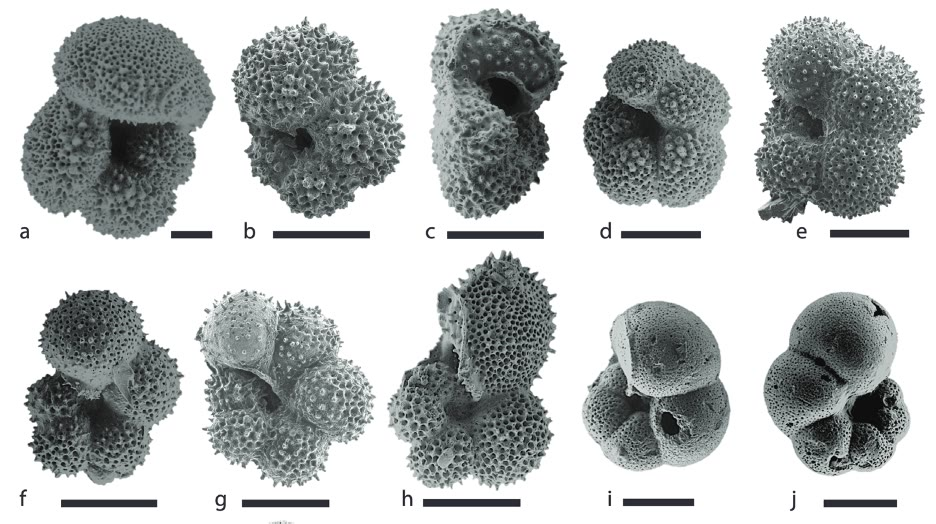
\includegraphics[width=0.62\linewidth]{images/book2/g12-planktic-foraminifera.jpg}

{\small 十个有孔虫物种的壳体，它们生活时漂浮于
海洋中；用扫描电子显微镜观察，每条线段比例尺为
\qty{150}{\micro\metre}，因此每个壳体约与一粒沙子大小相当。
Marci Robinson, USGS（公有领域，经由维基共享资源）。}
\end{omfigure}
% ledger: photo:g12-forams

壳体中的氧来自海水。由轻同位素氧-16 构成的水
更易蒸发，因此形成冰盖的
降雪中氧-18 含量偏低。冰盖增长时，它们储存这些轻水，
留下的海洋便富含氧-18；生长于其中的壳体也是如此，
水温越低，富集越明显。海底有孔虫壳体中氧-18 的占比，
记为 $\delta^{18}\mathrm{O}$，以千分之一表示，
因而可作为陆地冰量与\omterm{def:g10:layered-ocean:thermocline}{深海}温度的\omterm{def:g12:past-climates:proxy}{代用指标}：
该值越高，
冰量越多，水温越低。
% ledger: nasaeo:o18, lr04:stack

下图所示的记录称为 LR04，它将来自各大洋的
57 个岩芯的测量数据叠加成一条长 530 万年的曲线。

\begin{omfigure}
\begin{tikzpicture}
\begin{axis}[omrecord, scale only axis, width=0.86\linewidth, height=4.8cm,
  xmin=0, xmax=5.32, x dir=reverse, ymin=2.4, ymax=5.3, y dir=reverse,
  xtick={0,0.5,...,5}, ytick={2.5,3,...,5},
  x tick label style={/pgf/number format/.cd, fixed, precision=1},
  y tick label style={/pgf/number format/.cd, fixed, fixed zerofill, precision=1},
  xlabel={1950 年以前的百万年数},
  ylabel={壳体中的 $\delta^{18}\mathrm{O}$（\unit{\permil}）}]
\fill[omProp!14] (axis cs:1.25,2.4) rectangle (axis cs:0.7,5.3);
% data:lr04 (the stack only; ice_age_records.py)
\addplot[omDef!85!black, line width=0.35pt] table[x=age_Ma, y=d18O] {figdata/out/grade-12-ice_age_records-lr04.dat};
\addplot[omThm, line width=1pt, densely dashed, unbounded coords=jump] table[x=age_Ma, y=d18O] {figdata/out/grade-12-ice_age_records-lr04mean.dat};
\coordinate (mpt) at (axis cs:0.975,2.45);
\coordinate (mm) at (axis cs:5.22,4.92);
\coordinate (arr) at (axis cs:5.12,3.9);
\end{axis}
\node[font=\scriptsize, anchor=north, align=center] at (mpt) {41 000 至 \\100 000 年};
\draw[omThm, line width=1pt, densely dashed] (mm) -- ($(mm)+(0.5,0)$) node[right, font=\scriptsize, text=omThm] {530 万至 300 万年前与 100 万至 0 年前的均值};
\draw[-{Stealth}, black!70] (arr) -- ++(0,-0.9) node[midway, right, font=\scriptsize, align=left] {冰量增多，\\水温更低};
\end{tikzpicture}

{\small 海底有孔虫壳体中记录的五百万年
\omterm{def:g10:layered-ocean:thermocline}{深海}状况；纵轴方向颠倒，使寒冷\omterm{def:g12:past-climates:glacial-cycle}{冰期}位于
低处。虚线为前段和后段的均值。阴影部分表示
由 \num{41000} 年旋回向约 \num{100000} 年旋回的转变。
数据来源：Lisiecki 和 Raymo（2005），LR04 叠加曲线。}
\end{omfigure}
% ledger: data:lr04, lr04:stack, clark06:mpt

依上述方法读取该记录，可得三点结论。
\begin{itemize}
  \item \emph{地球已经变冷，冰量已经增加。}平均值
        由 530 万至 300 万年前的 \qty{3.03}{\permil}，
        上升为过去一百万年的 \qty{4.15}{\permil}。
  \item \emph{波动幅度加大。}\omterm{def:g12:past-climates:glacial-cycle}{冰期}与\omterm{def:g12:past-climates:glacial-cycle}{间冰期}
        贯穿整个记录交替出现，但波幅越来越大：在
        \omterm{def:g12:past-climates:lgm}{末次盛冰期}，数值为 \qty{4.92}{\permil}，
        而今天为 \qty{3.23}{\permil}。
  \item \emph{旋回节律发生了变化。}在 260 万至 130 万年前，
        记录中最强的周期，据其数据计算为 \num{41000} 年；
        而在过去 \num{700000} 年间约为
        \num{98000} 年，与\omterm{def:g12:past-climates:ice-core}{冰芯}所示节律一致。这一变化
        发生于约 125 万至 70 万年前。
\end{itemize}
% ledger: data:lr04, clark06:mpt (ice_age_records.py: lr04_mean_3_5Ma 3.032, lr04_mean_0_1Ma 4.147, lr04_lgm 4.92, lr04_today 3.23, periods 41.0 and 98.5 kyr)

这些周期并非偶然。1976 年，詹姆斯·海斯、约翰·因布里和尼古拉斯·
沙克尔顿在南部海洋的沉积物中发现了三种节律，
周期分别为 \num{23000}、\num{42000} 和约 \num{100000} 年，
它们正是地球轨道和自转轴缓慢变化的周期：自转轴的岁差、
自转轴倾角（约 \num{41000} 年）和轨道形状
（约 \num{100000} 年）。这些变化改变了各纬度
在各季节所接收的阳光，并由此决定\omterm{def:g12:past-climates:glacial-cycle}{冰期
旋回}的节奏。其作用方式，以及缓慢的 \num{100000} 年节律为何
能占据主导，属于大学课程的内容。
% ledger: hays76:periods, nasa:milankovitch, lr04:stack, clark06:mpt

\begin{dated}{2025}
2025 年 1 月，Beyond EPICA 项目宣布，在 Little Dome~C 钻取的一根岩芯，
距 Dome~C 上 Concordia 站约 \qty{35}{km}，其上部
\qty{2480}{m} 中的连续记录可追溯至约 120 万年前。该岩芯
覆盖的时段，正是\omterm{def:g12:past-climates:glacial-cycle}{冰期}节律由 \num{41000} 年
转变为 \num{100000} 年的时期，此时冰及其所含空气
正在接受分析。
\end{dated}
% ledger: ku25:beyond-epica, ipev25:little-dome-c

\section{远古气候}

比\omterm{def:g12:past-climates:ice-core}{冰芯}更久远的气候，需从沉积物、化石
叶片、土壤与同位素中读取。IPCC 已选定若干
\emph{参考时段}，研究充分，其气候有助于判断
当今及未来的气候变化。下图给出了它们的全球
地表温度，相对 1850--1900 年。

\begin{omfigure}
\begin{tikzpicture}
\begin{axis}[omrecord, width=0.86\linewidth, height=5.4cm, xmin=-9, xmax=27,
  ymin=0.4, ymax=6.6, y dir=reverse, ytick={1,...,6}, ymajorgrids=false,
  yticklabels={{PETM, 56 Ma}, {EECO, 53--49 Ma}, {MPWP, 3.3--3.0 Ma},
    {LIG, 129--116 ka}, {LGM, 23--19 ka}, {MH, 6.5--5.5 ka}},
  y tick label style={font=\scriptsize},
  xlabel={相对 1850--1900 年的温度（\unit{\degreeCelsius}）}]
% ipcc:fig2-34 (DEEP in ice_age_records.py)
\addplot[draw=none, mark=none, restrict expr to domain={\thisrow{tlo}}{0:30},
  error bars/.cd, x dir=both, x explicit,
  error bar style={line width=5pt, omWarm!75}, error mark=none]
  table[x expr={(\thisrow{tlo}+\thisrow{thi})/2}, y=idx,
        x error expr={(\thisrow{thi}-\thisrow{tlo})/2}] {figdata/out/grade-12-ice_age_records-deep.dat};
\addplot[draw=none, mark=none, restrict expr to domain={\thisrow{tlo}}{-30:-0.01},
  error bars/.cd, x dir=both, x explicit,
  error bar style={line width=5pt, omCold!75}, error mark=none]
  table[x expr={(\thisrow{tlo}+\thisrow{thi})/2}, y=idx,
        x error expr={(\thisrow{thi}-\thisrow{tlo})/2}] {figdata/out/grade-12-ice_age_records-deep.dat};
\draw[black!60] (axis cs:0,0.4) -- (axis cs:0,6.6);
\draw[omThm, densely dashed, line width=0.8pt] (axis cs:1.09,0.4) -- (axis cs:1.09,6.6);
\node[font=\scriptsize, text=omThm, anchor=west, fill=white, inner sep=1pt] at (axis cs:1.6,4.55) {2011--2020};
\end{axis}
\end{tikzpicture}

{\small 过去六个参照时期的全球表面温度，
很可能范围，相对于 1850--1900 年；虚线：2011--2020 年这一十年。
PETM：古新世–始新世极热事件；EECO：早始新世
气候最适期；MPWP：中上新世暖期；LIG：末次\omterm{def:g12:past-climates:glacial-cycle}{间冰期}；LGM：\omterm{def:g12:past-climates:lgm}{末次
盛冰期}（唯一的寒冷时期，蓝色）；MH：
全新世中期。数据来源：IPCC AR6 WG1 图 2.34。}
\end{omfigure}
% ledger: ipcc:fig2-34, ipcc:gsat-2011-2020, ipcc:ref-periods

\begin{center}
\small
\begin{tabular}{|l|c|c|c|}
\hline
\textbf{时期} & \textbf{温度（\unit{\degreeCelsius}）} & \textbf{二氧化碳（ppm）} & \textbf{海平面（m）} \\
\hline
PETM，56 Ma & $+10$ 至 $+25$ & 约 900，升至 2000 &——\\
EECO，53--49 Ma & $+10$ 至 $+18$ & 1150 至 2500 & $+70$ 至 $+76$ \\
MPWP，3.3--3.0 Ma & $+2.5$ 至 $+4.0$ & 360 至 420 & $+5$ 至 $+25$ \\
LIG，129--116 ka & $+0.5$ 至 $+1.5$ & 266 至 282 & $+5$ 至 $+10$ \\
\textcolor{omCold}{LGM，23--19 ka} & \textcolor{omCold}{$-7$ 至 $-5$} & \textcolor{omCold}{188 至 194} & \textcolor{omCold}{$-134$ 至 $-125$} \\
MH，6.5--5.5 ka & $+0.2$ 至 $+1.0$ & 260 至 268 & $-3.5$ 至 $+0.5$ \\
\hline
\end{tabular}

\medskip
{\small 参照时期的全球表面温度（相对于
1850--1900 年）、二氧化碳及全球海平面（相对于 1900 年）。IPCC
AR6 WG1 图 2.34。}
\end{center}
% ledger: ipcc:fig2-34

古新世–始新世极热事件是一次突然的变暖，当时大量
碳脉冲进入海洋与大气：海洋酸性增强，
氧含量降低，许多\omterm{def:g10:layered-ocean:thermocline}{深海}物种灭绝。早始新世
气候最适期，二氧化碳含量在 \qty{1000}{ppm} 以上持续了
数百万年，极地无冰，接近热带的森林
生长于南纬 \ang{70}。中上新世暖期是二氧化碳
含量接近今天水平的最后时期：北极比现在暖得多，海平面
比现在高。在末次\omterm{def:g12:past-climates:glacial-cycle}{间冰期}，格陵兰和西南极冰
盖更小，海平面高于今天，河马曾生活
在英国。
% ledger: ipcc:ref-periods, ipcc:fig2-34, ipcc:mpwp-eeco

这些档案为今天提供了参照，IPCC 本身也
进行了这一比较。2019 年，大气中的二氧化碳含量高于
至少两百万年中的任何时期（\emph{高信度}），且自 1750 年以来，二氧化碳
和甲烷的上升量远超过\omterm{def:g12:past-climates:glacial-cycle}{冰期}与\omterm{def:g12:past-climates:glacial-cycle}{间冰期}之间
的自然变化，时间跨度至少 \num{800000} 年（\emph{很高
信度}）。自 1970 年以来，全球表面温度的上升速度快于
至少过去 \num{2000} 年中任何其他 50 年的时段
（\emph{高信度}）。2011--2020 年这十年
比当前\omterm{def:g12:past-climates:glacial-cycle}{间冰期}约 \num{6500} 年前最暖的几个世纪更暖，且
接近末次\omterm{def:g12:past-climates:glacial-cycle}{间冰期}约 \num{125000} 年前的暖度
（\emph{中等信度}）。
% ledger: ipcc:co2-ch4-800kyr, ipcc:fastest-2000yr, ipcc:co2-2myr

变化速度也可以进行比较。从 1970 年到 2025 年，全球温度记录的趋势
为 \qty{0.20}{\degreeCelsius} 每十年，或者
约 \qty{20}{\degreeCelsius} 每千年（若保持该速率）；
末次\omterm{def:g12:past-climates:glacial-cycle}{冰期}结束后的升温平均约
\qty{0.86}{\degreeCelsius} 每千年。当今变化的成因，
及其可能的走向，将在\cref{ch:g12:climate-change}中讨论。
% ledger: data:gistemp (ice_age_records.py: rate_1970_2025_C_per_decade 0.2012), ipcc:lgm-cooling, ipcc:ref-periods

\section{练习}

\begin{exercise}[$\star$]\label{exo:g12:past-climates:1}
写出下列描述对应的术语：(a) 档案中测得的、用以代替
无法直接测量的气候变量的量；(b) 从冰盖中钻取的圆柱形冰样；
(c) 两次\omterm{def:g12:past-climates:glacial-cycle}{冰期}之间的温暖间期；(d) 由化石花粉重建
古植被；(e) 末次冰盖最大的时期，约 \num{23000} 至 \num{19000}
年前。
\end{exercise}

\begin{exercise}[$\star$]\label{exo:g12:past-climates:2}
对每个\omterm{def:g12:past-climates:proxy}{代用指标}，写出其所在档案及所反映的信息：(a) 气泡中的
空气；(b) 橡树花粉所占比例；(c) 海底有孔虫壳体的
氧-18 含量；(d) 树木年轮的宽度。
\end{exercise}

\begin{exercise}[$\star$]\label{exo:g12:past-climates:3}
在末次冰消期，即约 \num{18000} 至 \num{11000}
年前，海平面由约 \qty{-120}{m} 上升至 \qty{-50}{m}。(a) 计算
海平面上升的平均速率，单位为毫米每年。(b) 从 2006 年到 2018 年，海平面
每年上升 \qty{3.7}{mm}。比较两者。
\end{exercise}

\begin{exercise}[$\star$]\label{exo:g12:past-climates:4}
自 1970 年至 2025 年，全球温度每十年上升
\qty{0.20}{\degreeCelsius}。将此速率换算为每世纪和每千年。
\end{exercise}

\begin{exercise}[$\star$]\label{exo:g12:past-climates:5}
海斯、因布里和沙克尔顿在海洋沉积物中发现了三种节律：
周期分别为 \num{23000}、\num{42000} 和约 \num{100000} 年。(a) 将每一个周期与
地轴岁差、地轴倾角和轨道形状一一对应。
(b) \num{1000000} 年内可容纳多少个 \num{41000} 年的旋回？有多少个
\num{100000} 年的旋回？
\end{exercise}

\begin{exercise}[$\star\star$]\label{exo:g12:past-climates:6}
本章的最小二乘直线为 $\mathrm{CO_2} \approx 266.6 +
7.83\,\Delta T$（ppm，$\Delta T$ 单位为 \unit{\degreeCelsius}）。
(a) 预测\omterm{def:g12:past-climates:lgm}{末次盛冰期}
Dome~C 处的平均温度 \qty{-9.4}{\degreeCelsius} 时的二氧化碳含量，并与实测的
\qty{190}{ppm} 比较。(b) 预测最暖点 \qty{+5.5}{\degreeCelsius} 时的
二氧化碳含量，并与实测最高值 \qty{299}{ppm} 比较。(c) 利用该直线
估计 Dome~C 处与 \qty{427}{ppm} 对应的温度，该值为
2025 年莫纳罗亚站的观测值。为何这种用法不合理？
\end{exercise}

\begin{exercise}[$\star\star$]\label{exo:g12:past-climates:7}
用瓦尔登丘陵湖泊的\omterm{def:g12:past-climates:pollen}{孢粉图谱}。(a) 在 \qty{580}{cm} 处占优势的
花粉是什么，它指示何种景观？(b) 对 \qty{340}{cm} 处提出同样的
问题。(c) 冷期之后哪种树木最先扩散，哪些树木最后到达？
(d) 树木的到达为何可能滞后于
使其得以生长的变暖？
\end{exercise}

\begin{exercise}[$\star\star$]\label{exo:g12:past-climates:8}
在同一岩芯中，\qty{600}{cm} 处的泥层年龄为 \num{14000} 年，
而 \qty{300}{cm} 处的为 \num{6000} 年，沉积速率恒定。
(a) 以毫米每年为单位计算该速率。(b) 求 2 带与 3 带之间界限的年龄，
该界限位于 \qty{470}{cm} 处。(c) 一片厚
\qty{1}{cm} 的\omterm{def:g11:minerals:thin-section}{薄片}代表多少年？
\end{exercise}

\begin{exercise}[$\star\star$]\label{exo:g12:past-climates:9}
在东南亚地图上，海面下降 \qty{130}{m} 时，海面以上的陆地面积
由 4.11 百万平方千米增至 7.16 百万平方千米。
(a) 计算增加量及其百分比。(b) 在地图上，海面下降约
\qty{36}{m} 即可使婆罗洲与亚洲相连。该岛在整个\omterm{def:g12:past-climates:lgm}{末次
盛冰期}期间是否一直与亚洲相连？请说明理由。(c) 地图上的海岸线为何只是
近似的？
\end{exercise}

\begin{exercise}[$\star\star$]\label{exo:g12:past-climates:10}
在 LR04 记录中，\omterm{def:g12:past-climates:lgm}{末次盛冰期}的数值为
\qty{4.92}{\permil}，今天的数值为 \qty{3.23}{\permil}。(a) 哪个更高，
这是否符合预期？请结合冰盖加以解释。(b) 为何该记录的
纵轴要倒置绘制？
\end{exercise}

\begin{exercise}[$\star\star$]\label{exo:g12:past-climates:11}
某位朋友说：“南极温度与二氧化碳之间的相关系数为 0.92，
这证明二氧化碳控制了\omterm{def:g12:past-climates:glacial-cycle}{冰期}。”(a) 相关性说明了什么，又不能说明什么？
(b) 给出两种能产生同样相关性的其他解释。
(c) 哪一类关于两份记录的
信息有助于作出判断？
\end{exercise}

\begin{exercise}[$\star\star\star$]\label{exo:g12:past-climates:12}
LR04 记录中最强的周期为 \num{41000} 年，出现在 260 万
至 130 万年前之间，而在最近 \num{700000} 年内则为 \num{98500} 年。
(a) 每个时段包含多少个循环？(b) 地球的哪种轨道或自转轴变化
与各周期相对应？(c) 请解释为何每 \num{2000} 年取一个样本的记录
能够显示这些节律，却无法显示持续一个世纪的
变化。
\end{exercise}

\begin{exercise}[$\star\star\star$]\label{exo:g12:past-climates:13}
二氧化碳的上升速率在 1995--2014 年间为每世纪 192 至
\qty{198}{ppm}。古新世–始新世极热事件期间为每世纪 4 至
\qty{42}{ppm}，末次冰消期过渡阶段的上升速率至多约为
每世纪 \qty{10}{ppm}。(a) 近期的上升速率是末次冰消期最快上升速率的多少倍？
(b) 相比古新世–始新世极热事件中最慢与最快的估计值，分别是多少倍？
(c) 古新世–始新世极热事件中的升高由约 900 ppm 升至约
\qty{2000}{ppm}。若按每世纪 \qty{42}{ppm} 的速率，需要多少时间？
若按今天的速率，又需要多少时间？
\end{exercise}

\begin{exercise}[$\star\star\star$]\label{exo:g12:past-climates:14}
IPCC 估计，全球温度在末次冰消期最快的阶段每千年上升 1 至
\qty{1.5}{\degreeCelsius}，而格陵兰上空在变暖最剧烈的
数个世纪中升温速率约快十倍。(a) 给出格陵兰的升温速率，
分别以 \unit{\degreeCelsius} 每千年和每十年为单位。
(b) 将其与今日全球 \qty{0.20}{\degreeCelsius} 每十年的速率相比。
(c) 为何局地速率
不能直接与全球速率比较？
\end{exercise}

\begin{exercise}[$\star\star\star$]\label{exo:g12:past-climates:15}
约 \num{11000} 年前海平面约为 \qty{-50}{m}，假设此后海平面
以稳定速率每千年上升 \qty{12}{m}，即主要冰消期的平均速率。
(a) 海平面何时越过 \qty{-36}{m}，即地图上使婆罗洲
与亚洲相连的水位？(b) 此后某人能否从婆罗洲步行至马来半岛？
(c) 若海平面以相同速度继续上升，
上升最后 \qty{36}{m} 需要多长时间？
\end{exercise}

\begin{problem}[{周末问题——南极冰芯中的 800 000 年}]
\label{pb:g12:past-climates:1}
% ledger: data:edc-jouzel, data:co2-bereiter, data:lr04, data:gistemp, ipcc:lgm-cooling, ipcc:ref-periods, hays76:periods, clark06:mpt
% values (ice_age_records.py): edc -10.58 / +5.46, co2 173.71 / 298.6, r 0.9165, fit 266.57 + 7.827 T,
% LGM -9.389 / 189.67, 11-9 ka -0.360 / 264.10, period 97.5, rate 0.2012 per decade, ratio 23.48
Dome~C 的冰及其气泡中的空气给出下列数值。
其中温度指冰层相对于最近一千年的变化量。

\begin{center}
\small
\begin{tabular}{|l|c|c|}
\hline
 & \textbf{温度变化（\unit{\degreeCelsius}）} & \textbf{二氧化碳（ppm）} \\
\hline
最冷值，约 \num{24000} 年前 & $-10.6$ &——\\
最暖值，约 \num{129000} 年前 & $+5.5$ &——\\
二氧化碳的最低值与最高值 &——& 174 与 299 \\
均值，\num{23000} 至 \num{19000} 年前 & $-9.4$ & 190 \\
均值，\num{11000} 至 \num{9000} 年前 & $-0.4$ & 264 \\
\hline
\end{tabular}
\end{center}

温度记录中最强的周期约为 \num{98000} 年，
由 1639 组数据对得到的相关系数为 0.92。

\medskip
\noindent\textbf{第一部分——读取两份记录。}
\begin{enumerate}
  \item \omterm{def:g12:past-climates:ice-core}{冰芯}的哪一部分记录温度，哪一部分记录
        二氧化碳？
  \item 计算 Dome~C 处温度变化的全部范围。
  \item 计算二氧化碳的全部范围。
  \item 相关系数 0.92 说明了这两份
        记录之间的什么关系？
  \item 在本章的时间轴图中，今天位于右侧。为何
        读此类图之前必须先检查时间的走向？
\end{enumerate}

\medskip
\noindent\textbf{第二部分——\omterm{def:g12:past-climates:glacial-cycle}{冰期}与\omterm{def:g12:past-climates:glacial-cycle}{间冰期}的数值。}
\begin{enumerate}[resume]
  \item 定义\omterm{def:g12:past-climates:glacial-cycle}{冰期}和\omterm{def:g12:past-climates:glacial-cycle}{间冰期}。
  \item 我们生活在两者中的哪一个时期？该时期自何时开始？
  \item \num{800000} 年中可容纳多少个 \num{98000} 年的循环？
  \item 地球轨道的哪一种变化，其周期接近
        \num{100000} 年？
  \item 在约 125 万年前以前，\omterm{def:g12:past-climates:glacial-cycle}{冰期旋回}的
        主要节律是什么？
\end{enumerate}

\medskip
\noindent\textbf{第三部分——末次冰消期。}
\begin{enumerate}[resume]
  \item 在\omterm{def:g12:past-climates:lgm}{末次盛冰期}与 \num{11000} 至 \num{9000}
        年前之间，Dome~C 上空的温度上升了多少？
  \item 同一时段内，二氧化碳上升了多少？
  \item \omterm{def:g12:past-climates:lgm}{末次盛冰期}的全球温度比 1850--1900 年低 5 至
        \qty{7}{\degreeCelsius}，取此范围的中值。
        南极的变化比该中值更大还是更小？
  \item 末次冰消过渡期自 \num{18000} 年前
        持续至 \num{11000} 年前，这段时间有多长？
  \item 计算该过渡期内全球变暖的平均速率，单位为
        \unit{\degreeCelsius} 每千年。
  \item 将此速率以 \unit{\degreeCelsius} 每十年表示。
\end{enumerate}

\medskip
\noindent\textbf{第四部分——今日速率的比较。}
\begin{enumerate}[resume]
  \item 1970 年至 2025 年间，全球温度每十年上升
        \qty{0.20}{\degreeCelsius}。将该速率
        换算为每千年的数值。
  \item 今日变暖速度是末次冰消期平均变暖速度的
        多少倍？
  \item 在冰消期变化最快的阶段，全球温度每千年上升 1 至
        \qty{1.5}{\degreeCelsius}。
        今日速率是这些速率的多少倍？
  \item 综上，今日全球变暖速度是
        末次\omterm{def:g12:past-climates:glacial-cycle}{冰期}结束后变暖速度的多少倍？
\end{enumerate}
\end{problem}
